% \begin{figure}
%     \centering
%     \includegraphics{figures/FID-vs-Params-Plot.eps}
%     \caption{This scatter-plot shows the FID performance of our model on FFHQ-256 vs the number of parameters when only trained for 5million steps}
%     \label{fig:fid-vs-params-ablation}
% \end{figure}


\section{A Roadmap to a New Baseline --- \modelName}
\label{sec:roadmap}

% \vk{What about naming the new GAN that is being proposed? SimpleGAN...?}\jt{R3GAN...?}

% \vk{My main comment about this section is that it reads like mix of methods and experiments: all the experimental details/results (e.g., we set the learning rate to $10^{-4}$) should be under experiments (but you can still describe the key important takeaways here, e.g., we need a smaller learning rate)}

The well-behaved RpGAN + $R_1$ + $R_2$ loss alleviates GAN optimization problems, and lets us proceed to build a minimalist baseline---\modelName---with recent network backbone advances in mind~\cite{convnext,metaformer}. Rather than simply state the new approach, we will draw out a roadmap from the StyleGAN2 baseline~\cite{sg2ada}. This model (Config A; identical to~\cite{sg2ada}) consists of a VGG-like~\cite{vgg} backbone for $G$, a ResNet $D$, a few techniques that facilitate style-based generation, and many tricks that serve as patches to the weak backbone. Then, we remove all non-essential features of StyleGAN2 (Config B), apply our loss function (Config C), and gradually modernize the network backbone (Config D-E).


We evaluate each configuration on FFHQ $256\times256$~\cite{sg1}. Network capacity is kept roughly the same for all configurations---both $G$ and $D$ have about 25M trainable parameters. Each configuration is trained until $D$ sees 5M real images. We inherit training hyperparameters (optimizer settings, batch size, EMA decay length,~\etc) from Config A unless otherwise specified. We tune the training hyperparameters for our final model and show the converged result in Sec.~\ref{sec:exp}.

%\paragraph{StyleGAN2 (Config A).}This configuration is identical to the baseline~\cite{sg2ada} with the style-based generator and all tricks enabled.  

\vspace{-1ex}
\paragraph{Minimum Baseline (Config B).}
We strip away all StyleGAN2 features, retaining only the raw network backbone and basic image generation capability. The features fall into three categories:
\begin{itemize}[leftmargin=10pt,itemsep=0pt,topsep=0pt]
\item Style-based generation: mapping network~\cite{sg1}, style injection~\cite{sg1}, weight modulation/demodulation~\cite{sg2}, noise injection~\cite{sg1}.
\end{itemize}\quad % JT: Weird but intential LaTeX
\begin{itemize}[leftmargin=10pt,itemsep=0pt,topsep=0pt]
\vspace{-0.25cm} % JT: Weird but intential LaTeX
\item Image manipulation enhancements: mixing regularization~\cite{sg1}, path length regularization~\cite{sg2}.
\item Tricks: $z$ normalization~\cite{pggan}, minibatch stddev~\cite{pggan}, equalized learning rate~\cite{pggan}, lazy regularization~\cite{sg2}.
\end{itemize}

% Such features could be reintroduced as per application need (e.g., style injection). 
Following~\cite{sgxl,sg-t}, we reduce the dimension of $z$ to 64. The absence of equalized learning rate necessitates a lower learning rate, reduced from $2.5\times10^{-3}$ to $5\times10^{-5}$. Despite a higher FID of 12.46 than Config-A, this simplified baseline produces reasonable sample quality and stable training. We compare this with DCGAN~\cite{dcgan}, an early attempt at image generation. Key differences include:
\begin{enumerate}[label=\alph*), noitemsep,topsep=0pt,leftmargin=24pt]
\item Convergent training objective with $R_1$ regularization.\label{item:convergent} 
\item Smaller learning rate, avoiding momentum optimizer (Adam $\beta_1=0$).\label{item:learning_rate} 
\item No normalization layer in $G$ or $D$.\label{item:normalization} 
\item Proper resampling via bilinear interpolation instead of strided (transposed) convolution.\label{item:resampling} 
\item Leaky ReLU in both $G$ and $D$, no tanh in the output layer of $G$.\label{item:activation} 
\item $4\times4$ constant input for $G$, output skips for $G$, ResNet $D$.\label{item:input} 
\end{enumerate}

We discuss our findings about these principles in Appendix B and establish that \ref{item:convergent} through \ref{item:activation} are critical to the success of StyleGAN2, and apply them to all subsequent configurations.

\paragraph{Well-behaved loss function (Config C).}
% Given the simplified baseline, we move on to the modernization part of the roadmap. We first modernize the loss function so that the representation power of modern network backbones will not be compromised by GAN optimization difficulties. 
We use the loss function proposed in Section~\ref{sec:loss} and this reduces FID to 11.65. We hypothesize that the network backbone in Config B is the limiting factor. 
% and expect more drastic improvements as further modernization takes place.

\paragraph{General network modernization (Config D).}
First, we apply the 1-3-1 bottleneck ResNet architecture~\cite{resnet,resnet2} to both $G$ and $D$. This is the direct ancestor of all modern vision backbones~\cite{convnext,metaformer}. 
% However, rather than precisely replicating the architecture in~\cite{resnet2}, 
We also incorporate principles discovered in Config B and various modernization efforts from ConvNeXt~\cite{convnext}. We categorize the roadmap of ConvNeXt as follows:
% \begin{enumerate}[label=\roman*)]
%     \item Consistently beneficial: 1) increased width with depthwise conv. 2) inverted bottleneck. 3) fewer activation functions. 4) separate resampling layers.
%     \item Negligible performance gain: 1) large kernel depthwise conv with fewer channels. 2) replacing ReLU with GELU. 3) fewer normalization layers. 4) replacing batch norm with layer norm.
%     \item Irrelevant to our problem setting: 1) improved training recipe. 2) stage ratio. 3) "patchify" stem.
% \end{enumerate}
% % We are interested in applying i) to our model, among which i.3) and i.4) are applicable to the classic ResNet. We leave i.1) and i.2) for Config E. Much of ii) were introduced merely for the sake of mimicking vision transformers~\cite{swin,vit} even though they fail to bring any significant improvement~\cite{convnext}. ii.3) and ii.4) are inapplicable since we do not use any normalization layer following principle c). ii.2) is directly at odds with our finding that GELU deteriorates GAN performance, and we use leaky ReLU as in principle e). Liu~\etal put heavy emphasis on using large conv kernels (ii.1)~\cite{convnext}, however this results in slightly but consistently worse performance than using wider $3\times3$ conv layers and we therefore do not employ this design choice of ConvNeXt.

% We aim to apply i) to our model, specifically i.3) and i.4) for the classic ResNet, while reserving i.1) and i.2) for Config E. Many aspects of ii) were introduced merely to mimic vision transformers~\cite{swin,vit} without yielding significant improvements~\cite{convnext}. ii.3) and ii.4) are inapplicable due to our avoidance of normalization layers following principle c). ii.2) contradicts our finding that GELU deteriorates GAN performance, thus we use leaky ReLU per principle e). Liu~\etal emphasize large conv kernels (ii.1)~\cite{convnext}, but this results in slightly worse performance compared to wider $3\times3$ conv layers, so we do not adopt this ConvNeXt design choice.
%
\begin{enumerate}[label=\roman*., itemsep=2pt,leftmargin=12pt,topsep=0pt]
    \item Consistently beneficial: \begin{enumerate*}[label=\theenumi\arabic*), ref=\arabic*, before=\unskip{ }, itemjoin={{, }}, itemjoin*={{, and }}]
        \item\label{item:i1} increased width with depthwise conv.
        \item\label{item:i2} inverted bottleneck
        \item\label{item:i3} fewer activation functions
        \item\label{item:i4} separate resampling layers
    \end{enumerate*}
    \item Negligible performance gain: \begin{enumerate*}[label=\theenumi\arabic*), ref=\arabic*, before=\unskip{ }, itemjoin={{, }}, itemjoin*={{, and }}]
        \item\label{item:ii1} large kernel depthwise conv.~with fewer channels
        \item\label{item:ii2} swap ReLU with GELU
        \item\label{item:ii3} fewer normalization layers
        \item\label{item:ii4} swap batch norm.~with layer norm.
    \end{enumerate*}
    \item Irrelevant to our setting: \begin{enumerate*}[label=\theenumi\arabic*), ref=\arabic*, before=\unskip{ }, itemjoin={{, }}, itemjoin*={{, and }}]
        \item\label{item:iii1} improved training recipe
        \item\label{item:iii2} stage ratio
        \item\label{item:iii3} ``patchify'' stem
    \end{enumerate*}
\end{enumerate}

We aim to apply i) to our model, specifically i.\ref{item:i3} and i.\ref{item:i4} for the classic ResNet, while reserving i.\ref{item:i1} and i.\ref{item:i2} for Config E. Many aspects of ii) were introduced merely to mimic vision transformers~\cite{swin,vit} without yielding significant improvements~\cite{convnext}. ii.\ref{item:ii3} and ii.\ref{item:ii4} are inapplicable due to our avoidance of normalization layers following principle c). ii.\ref{item:ii2} contradicts our finding that GELU deteriorates GAN performance, thus we use leaky ReLU per principle e). Liu~\etal emphasize large conv kernels (ii.\ref{item:ii1})~\cite{convnext}, but this results in slightly worse performance compared to wider $3\times3$ conv layers, so we do not adopt this ConvNeXt design choice. We discuss the architecture details in Appendix C.

\begin{figure}[t]
    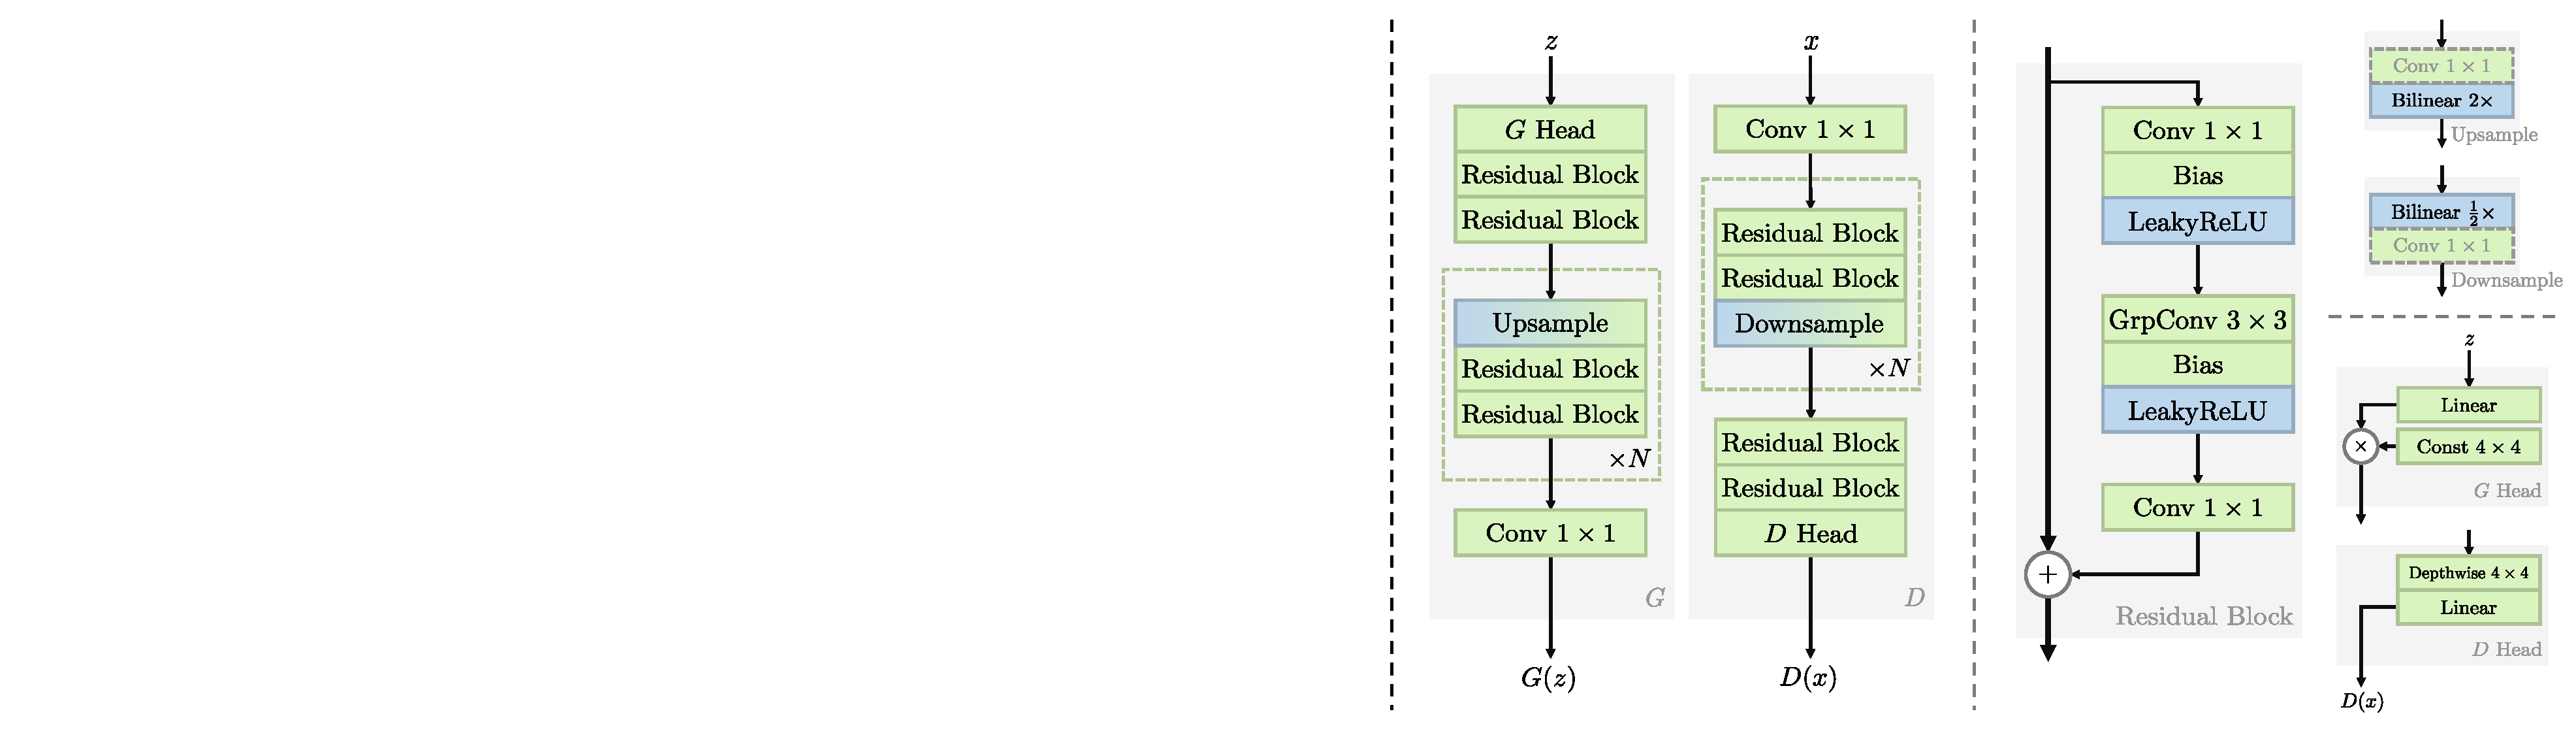
\includegraphics[width=\linewidth,clip,trim={87pc 0cm 0cm 0cm}]{figures/network.pdf}
    \caption{Network architecture blocks.}
    \label{fig:network}
    \vspace{-0.7cm}
\end{figure}

\paragraph{Bottleneck modernization (Config E).}
Now that we have settled on the overall architecture, we investigate how the residual block can be modernized, specifically i.\ref{item:i1}) and i.\ref{item:i2}). First, we explore i.\ref{item:i1} and replace the $3\times3$ convolution in the residual block with a grouped convolution. We set the group size to 16 rather than 1 (\ie depthwise convolution as in ConvNeXt) as depthwise convolution is highly inefficient on GPUs and is not much faster than using a larger group size. With grouped convolution, we can reduce the bottleneck compression ratio to two given the same model size. This increases the width of the bottleneck to $1.5\times$ as wide as Config A. 
%With this, the FID drops to 7.51, surpassing the performance of StyleGAN2. 
Finally, we notice that the compute cost of grouped convolution is negligible compared to $1\times1$ convolution, and so we seek to enhance the capacity of grouped convolution. We apply i.\ref{item:i2}), which inverts the bottleneck width and the stem width, and which doubles the width of grouped convolutions without any increase in model size. Figure~\ref{fig:network} depicts our final design, which reflects modern CNN architectures.
